\documentclass[12pt]{article}
\usepackage[a4paper,top=3cm,bottom=2cm,left=2cm,right=2cm,marginparwidth=1.2cm]{geometry}
\usepackage{fancyhdr}
\usepackage{pgfplots}
\usepackage{caption}
\usepackage{xcolor}
\usepackage{mdframed}
\usepgfplotslibrary{fillbetween}
\pgfplotsset{compat=1.18}
\usepackage{float}

\author{Eden Li}
\title{STAT110/115 Tutoring Materials – 02 R Functions and Tests}
\date{}

\begin{document}
\pagestyle{fancy}
\lhead{STAT110/115 Tutoring Materials}
\rhead{R Functions}

\begin{itemize}
\item \textbf{Usage of pnorm()}: pnorm(q, mean = 0, sd = 1, lower.tail = TRUE)

\begin{figure} [H]
\centering
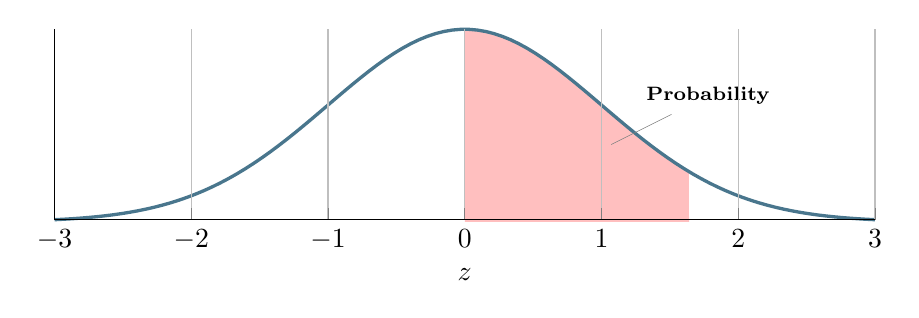
\begin{tikzpicture}

    \begin{axis}[
        no markers, 
        domain=-3:3, 
        samples=100, 
        axis lines*=left, 
        xlabel=$z$, 
        height=4cm, 
        width=12cm, 
        xtick={-3,-2,-1,0,1,2,3}, 
        ytick=\empty,
        enlargelimits=false, 
        clip=false, 
        axis on top,
        grid = major
    ]
    \addplot [very thick,cyan!50!black] {exp(-x^2/2)/sqrt(2*pi)};
    \addplot [name path=A,domain=0:1.64,cyan!50!black] {exp(-x^2/2)/sqrt(2*pi)};
    \path [name path=B] (axis cs:0,0) -- (axis cs:1.64,0);
    \addplot [red!50,opacity=0.5] fill between[of=A and B];
    \node[pin=above right:{\scriptsize \textbf{Probability}}] at (axis cs:1,0.15) {};
    \end{axis}
\end{tikzpicture}

Find Pr(0 $<$ Z $<$ 1.64)\\
pnorm(1.64) - pnorm(0)
\end{figure}

This function is used to find the probability in a specific area under a normal distribution curve. The parameter 'q' is the "value" from which you want the area above/below. \\
Example question: Find the proportion of students with a height between 180-190cm.

\item \textbf{Usage of qnorm()}: qnorm(p, mean = 0, sd = 1, lower.tail = TRUE) 
\begin{figure} [H]
\centering
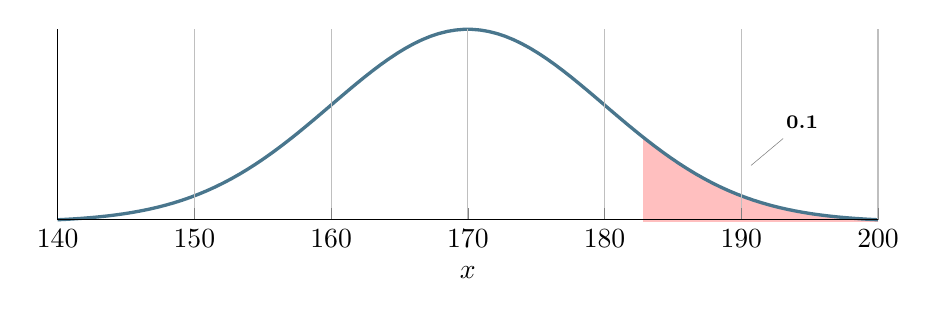
\begin{tikzpicture}
    \begin{axis}[
        no markers, 
        domain=-3:3, 
        samples=100, 
        axis lines*=left, 
        xlabel=$x$, 
        height=4cm, 
        width=12cm, 
        xtick={-3,-2,-1,0,1,2,3}, 
        xticklabels={140, 150, 160, 170, 180, 190, 200},
        ytick=\empty,
        enlargelimits=false, 
        clip=false, 
        axis on top,
        grid = major
    ]
    \addplot [very thick,cyan!50!black] {exp(-x^2/2)/sqrt(2*pi)};
    \addplot [name path=A,domain=1.282:3,cyan!50!black] {exp(-x^2/2)/sqrt(2*pi)};
    \path [name path=B] (axis cs:1.282,0) -- (axis cs:3,0);
    \addplot [red!50,opacity=0.5] fill between[of=A and B];
    \node[pin=above right:{\scriptsize \textbf{0.1}}] at (axis cs:2,0.1) {};
    \end{axis}
\end{tikzpicture}

Find the height which is exceeded by 10\% of students.\\
qnorm (0.1, mean = 170, sd=10, lower.tail = FALSE)\\
or\\
qnorm (0.9 ,mean = 170, sd = 10)\\
\end{figure}
This function is used to find the value "q" in pnorm(). \\
Example question: Find the height which is exceeded by 10\% of students.

\item \textbf{Usage of dbinom()}: dbinom(x=15, size=20, prob=0.75) \\
This function will provide the individual binomial probabilities associated with a given outcome, provided the number of trials (size) and the probability of 'success' (prob).

\item \textbf{Usage of pbinom()}: pbinom(q=10,size=20,prob=0.75) \\
This function will provide the sum of all individual binomial probabilities less than or equal to a given outcome q, provided the number of trials (size) and the probability of 'success' (prob). \\
Example question: Find the probability that 10 or fewer live with both parents.

\item \textbf{Usage of pt()}: 2*pt(q=2.12, df=17, lower.tail=FALSE)

\begin{figure} [H]
\centering
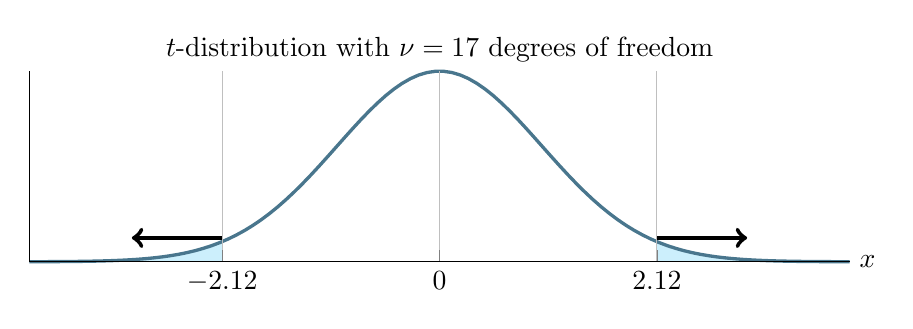
\begin{tikzpicture}
\begin{axis}[
    no markers, domain=-4:4, samples=100,
    axis lines*=left, xlabel=$x$, ylabel={$t$-distribution with $ \nu = 17 $ degrees of freedom},
    every axis y label/.style={at=(current axis.above origin),anchor=south},
    every axis x label/.style={at=(current axis.right of origin),anchor=west},
    height=4cm, width=12cm,
    xtick={-2.12,0,2.12}, ytick=\empty,
    enlargelimits=false, clip=false, axis on top,
    grid = major
]
\addplot [fill=cyan!20, draw=none, domain=-4:-2.12] {exp(-x^2/2)/sqrt(2*pi)} \closedcycle;
\addplot [fill=cyan!20, draw=none, domain=2.12:4] {exp(-x^2/2)/sqrt(2*pi)} \closedcycle;
\addplot [very thick,cyan!50!black] {exp(-x^2/2)/sqrt(2*pi)};

% Add arrows
\draw [->, ultra thick] (axis cs: -2.12,0.05) -- (axis cs: -3,0.05);
\draw [->, ultra thick] (axis cs: 2.12,0.05) -- (axis cs: 3,0.05);
\end{axis}
\end{tikzpicture}
\end{figure}

This function is used to get the p-value. Because there are two tails, so we need to *2.

\item \textbf{Usage of qt()}: qt(p, df) \\
This function is used to find the multiplier.

\item \textbf{Usage of pchisq()}: 1-pchisq(q = 9.70, df = 1) \\
This function is used to find the p-value of a chi-square.

\item \textbf{Usage of qchisq()}: qchisq(p = 0.95, df = 1) \\
This function is used to find the critical value of chi-square.

\item \textbf{Usage of pf()}: pf(1.0242, df1=3, df2=28, lower.tail=F) \\
This function is used to find the p-value of the F-distribution.

\item \textbf{Usage of qf()}: qf(0.05, 3, 15, lower.tail=FALSE) \\
This function is used to find the critical value of F statistic.

\item \textbf{Output for regression model fit}:

\begin{mdframed}[backgroundcolor=gray!15, linecolor=black]
\begin{verbatim}
Call:
lm(formula = y ~ x1 + x2, data = mydata)

Residuals:
    Min      1Q  Median      3Q     Max 
-1.1411 -0.3145  0.0187  0.3178  1.1867 

Coefficients:
            Estimate Std. Error t value Pr(>|t|)    
(Intercept)   2.2154     0.1321   16.77   <2e-16 ***
x1           -0.7307     0.0917   -7.97   <2e-16 ***
x2            0.3263     0.0862    3.78   <2e-16 ***

Signif. codes:  
*** p<0.001 ** p<0.01 * p<0.05 ' ' p>0.05

Residual standard error: 0.5209 on 37 degrees of freedom
Multiple R-squared: 0.7995, Adjusted R-squared: 0.7833 
F-statistic: 49.79 on 2 and 37 DF, p-value: 5.757e-11
\end{verbatim}
\end{mdframed}

\begin{itemize}
\item The "Residual standard error" represents the standard deviation of the residuals, which is an estimate of the average distance between the observed and predicted values.
\item The "Multiple R-squared" and "Adjusted R-squared" values indicate the goodness of fit of the model. They represent the proportion of variance in the response variable explained by the predictors. Adjusted R-squared takes into account the number of predictors and the sample size.
\item The "F-statistic" is a measure of the overall significance of the model. It assesses whether the regression model as a whole is statistically significant. 
\item The associated p-value indicates the probability of obtaining such an F-statistic by chance.
\end{itemize}

\item \textbf{Output for a t test}:

\begin{mdframed}[backgroundcolor=gray!15, linecolor=black]
\begin{verbatim}
Analysis of Variance Table

Response: y
             Df  Sum Sq Mean Sq F value Pr(>F)    
x1            1  1.3456  1.3456  12.463 0.00123 **
x2            2  0.7621  0.3811   3.527 0.03812 * 
Residuals    36  3.5584  0.0988                   

Signif. codes: 0 ‘***’ 0.001 ‘**’ 0.01 ‘*’ 0.05 ‘.’ 0.1 ‘ ’ 1
\end{verbatim}
\end{mdframed}

\begin{itemize}
\item The "data" line indicates the name of the variable or group being tested.
\item The "t" value represents the calculated t-statistic for the test. It measures the difference between the sample mean and the hypothesised mean relative to the variability in the data.
\item The "df" value stands for degrees of freedom, which measures the amount of information available for the test. It represents the sample size minus one.
\item The "p-value" is the probability of obtaining the observed test statistic (t-value) or a more extreme value under the null hypothesis. It indicates the level of statistical significance.
\item The "alternative hypothesis" states the alternative to the null hypothesis.
\item The "95 per cent confidence interval" provides a range of values within which we can be 95\% confident that the true population mean lies. It is calculated based on the sample data and reflects the estimate's precision.
\item The "sample estimates" section presents the estimated mean of the variable or group being tested.
\end{itemize}

\item \textbf{Output for an ANOVA table}:

\begin{mdframed}[backgroundcolor=gray!15, linecolor=black]
\begin{verbatim}
data: x

t = 3.5897, df = 98, p-value = 0.0005379

alternative hypothesis: true mean is not equal to 0

95 percent confidence interval:
 0.05743578 0.19679155

sample estimates:
mean of x
 0.1271137
\end{verbatim}
\end{mdframed}

\begin{itemize}
\item The "Response" line shows the name of the dependent variable.
\item The "Df" column represents the degrees of freedom associated with each factor or source of variation.
\item The "Sum Sq" column shows the sum of squares associated with each factor or source of variation. It represents the total variability explained by each factor.
\item The "Mean Sq" column represents the mean square, which is calculated by dividing the sum of squares by the degrees of freedom. It represents the average variability explained by each factor.
\item The "F value" column displays the F-statistic, which is calculated by dividing the mean square of each factor by the mean square of the residuals. It measures the ratio of explained variation to unexplained variation and is used to test the significance of each factor.
\item The "Pr($>$F)" column shows the p-value associated with each factor. It indicates the probability of obtaining the observed F-statistic or a more extreme value under the null hypothesis.
\end{itemize}
\end{itemize}

\end{document}
